\documentclass[11pt,a4paper]{article}

% Packages
\usepackage[utf8]{inputenc}
\usepackage[T1]{fontenc}
\usepackage{amsmath,amssymb,amsfonts}
\usepackage{graphicx}
\usepackage{booktabs}
\usepackage{hyperref}
\usepackage{xcolor}
\usepackage{float}
\usepackage{multirow}
\usepackage[margin=0.9in]{geometry}
\usepackage{caption}
\usepackage{subcaption}
\usepackage{enumitem}
\usepackage{algorithm}
\usepackage{algpseudocode}
\usepackage{longtable}
\usepackage{array}
\usepackage{tabularx}
\usepackage{fancyhdr}
\setlength{\headheight}{14pt}
\usepackage{lastpage}
\usepackage{titlesec}
\usepackage{listings}
\usepackage{tikz}
\usetikzlibrary{shapes.geometric, arrows.meta, positioning, calc, fit, backgrounds, decorations.pathreplacing}
\newcommand{\rupmark}{\textrm{INR}}

% Custom Colors for Code Listings
\definecolor{codegreen}{rgb}{0,0.6,0}
\definecolor{codegray}{rgb}{0.5,0.5,0.5}
\definecolor{codepurple}{rgb}{0.58,0,0.82}
\definecolor{backcolour}{rgb}{0.95,0.95,0.92}

% Python Code Style
\lstdefinestyle{custompython}{
    backgroundcolor=\color{backcolour},
    commentstyle=\color{codegreen},
    keywordstyle=\color{magenta},
    numberstyle=\tiny\color{codegray},
    stringstyle=\color{codepurple},
    basicstyle=\ttfamily\scriptsize,
    breakatwhitespace=false,
    breaklines=true,
    captionpos=b,
    keepspaces=true,
    numbers=left,
    numbersep=5pt,
    showspaces=false,
    showstringspaces=false,
    showtabs=false,
    tabsize=2,
    language=Python,
    frame=single
}

\lstset{style=custompython}

% Page style
\pagestyle{fancy}
\fancyhf{}
\fancyhead[L]{6th NHAI Innovation Hackathon 2026}
\fancyhead[R]{\thepage}
\fancyfoot[C]{Madhav Dogra | RetroGuard: AI-Powered Retroreflectivity Assessment}
\renewcommand{\headrulewidth}{0.4pt}
\renewcommand{\footrulewidth}{0.4pt}

% Colors
\definecolor{nhaiblue}{RGB}{0, 51, 153}
\definecolor{nhaiorange}{RGB}{255, 102, 0}
\definecolor{linkblue}{RGB}{0, 102, 204}
\definecolor{criticalred}{RGB}{220, 53, 69}
\definecolor{warningorange}{RGB}{255, 153, 0}
\definecolor{successgreen}{RGB}{40, 167, 69}
\definecolor{layerA}{RGB}{52, 152, 219}
\definecolor{layerB}{RGB}{46, 204, 113}
\definecolor{layerC}{RGB}{155, 89, 182}
\definecolor{layerD}{RGB}{230, 126, 34}
\definecolor{layerE}{RGB}{231, 76, 60}
\definecolor{layerF}{RGB}{241, 196, 15}
\definecolor{lightgray}{RGB}{245, 245, 245}
\definecolor{dashboardbg}{RGB}{236, 240, 241}

\hypersetup{
    colorlinks=true,
    linkcolor=linkblue,
    citecolor=linkblue,
    urlcolor=linkblue
}

% Graphics path
\graphicspath{{figures/}}

% Title formatting
\titleformat{\section}{\large\bfseries\color{nhaiblue}}{\thesection}{1em}{}
\titleformat{\subsection}{\normalsize\bfseries}{\thesubsection}{1em}{}

% Title
\title{
    \vspace{-1cm}
    \textbf{\LARGE RetroGuard: A Multi-Layered AI-Powered System for Automated Retroreflectivity Assessment on Indian National Highways}\\[0.5cm]
    \large Smartphone Measurement, CCTV Intelligence Mining, Crowdsourced Dashcam Networks, and Predictive Digital Twin for Highway Safety Asset Management\\[0.3cm]
    \textbf{6th NHAI Innovation Hackathon -- Problem Statement: Retroreflectivity Measurement}\\[0.5cm]
    \rule{\textwidth}{0.5pt}
}

\author{
    \textbf{Madhav Dogra}\\
    6th NHAI Innovation Hackathon 2026\\
    \texttt{madhavdogra@gmail.com}
}

\date{April 2026}

\begin{document}

\maketitle
\thispagestyle{empty}

% Abstract
\begin{abstract}
\noindent\textbf{Background:} The National Highways Authority of India (NHAI) manages over 1,40,000 km of national highways equipped with traffic signs, pavement markings, road studs (RPMs), and delineators. Retroreflectivity --- the ability of these safety assets to return light to its source --- is critical for driver visibility at night and in adverse weather. Current measurement relies on handheld retroreflectometers (per IRC~67 and IRC~35), a process that is slow ($\sim$2--5 measurements per hour for signs), dangerous on high-speed expressways, and fundamentally unscalable to the national highway network.

\noindent\textbf{Objective:} To design and prototype \textbf{RetroGuard}, a multi-layered, AI-powered system that automates retroreflectivity assessment using six complementary technologies, enabling continuous, network-wide monitoring with minimal new infrastructure investment.

\noindent\textbf{Approach:} RetroGuard operates through six synergistic layers: (1)~a \textbf{smartphone retroreflectometer} app using calibrated flash/camera optics; (2)~\textbf{existing CCTV footage mining} analyzing vehicle headlight reflections at night; (3)~\textbf{retroreflective reference patches} for universal camera calibration; (4)~a \textbf{crowdsourced dashcam intelligence network} leveraging fleet vehicles; (5)~a \textbf{predictive digital twin} with ML-based degradation forecasting; and (6)~\textbf{degradation-encoding QR codes} embedded during sign manufacturing. The AI pipeline employs YOLOv8/RT-DETR for object detection and a calibrated regression CNN for retroreflectivity coefficient ($R_L$) estimation.

\noindent\textbf{Key Innovation:} Each layer independently adds value using existing infrastructure, yet together they create a self-improving, predictive highway safety monitoring system that shifts maintenance from reactive to predictive --- potentially preventing the estimated 1,50,000 annual road fatalities attributable in part to degraded signage visibility.

\vspace{0.3cm}
\noindent\textbf{Keywords:} Retroreflectivity, Highway Safety, Computer Vision, YOLO, Digital Twin, Crowdsourcing, Smartphone Sensing, Predictive Maintenance, NHAI, IRC~67, IRC~35, Pavement Markings, Traffic Signs
\end{abstract}

\newpage
\tableofcontents
\newpage

%==============================================================================
\section{Introduction}
%==============================================================================

\subsection{The Retroreflectivity Imperative}

Road traffic accidents claim approximately 1,53,972 lives annually in India (MoRTH, 2023), with a disproportionate share occurring at night and during adverse weather conditions. A significant contributing factor is degraded visibility of road signs, pavement markings, and delineators. \textbf{Retroreflectivity} --- the optical property that enables these safety assets to return incident light from vehicle headlights back toward the driver --- is the single most important measurable characteristic that determines their nighttime effectiveness.

Retroreflectivity is quantified by the coefficient of retroreflected luminance $R_L$, defined as:

\begin{equation}
R_L = \frac{L}{E_\perp} \quad \left[\frac{\text{mcd}}{\text{lx} \cdot \text{m}^2}\right]
\label{eq:rl_definition}
\end{equation}

where $L$ is the luminance of the retroreflective surface as measured at the observation angle, and $E_\perp$ is the illuminance at the surface perpendicular to the incident light. For traffic signs, values of $R_A$ (coefficient of retroreflection) are used:

\begin{equation}
R_A = \frac{I}{E_\perp \cdot A} \quad \left[\frac{\text{cd}}{\text{lx} \cdot \text{m}^2}\right]
\label{eq:ra_definition}
\end{equation}

where $I$ is the luminous intensity of the retroreflected light and $A$ is the area of the retroreflective surface.

\subsection{Current Measurement Paradigm and Its Limitations}

NHAI mandates retroreflectivity measurement per two Indian Roads Congress standards:

\begin{itemize}[noitemsep]
    \item \textbf{IRC~67:} Code of Practice for Road Signs --- specifies minimum retroreflectivity for traffic signs using different grades of sheeting (Engineering Grade, High Intensity, Diamond Grade)
    \item \textbf{IRC~35:} Code of Practice for Road Markings --- specifies minimum retroreflectivity for pavement markings, road studs, and delineators
\end{itemize}

The current measurement workflow suffers from critical limitations:

\begin{table}[H]
\centering
\caption{Limitations of Current Handheld Retroreflectivity Measurement}
\label{tab:limitations}
\begin{tabular}{@{}p{3.5cm}p{10cm}@{}}
\toprule
\textbf{Limitation} & \textbf{Impact} \\
\midrule
\textbf{Speed} & 2--5 sign measurements per hour; marking measurements require stopping on the roadway \\
\textbf{Safety} & Inspector must stand on or beside high-speed expressways (80--120 km/h design speed) \\
\textbf{Coverage} & $<$1\% of highway assets measured during typical O\&M inspection cycles \\
\textbf{Cost} & Handheld retroreflectometers cost \rupmark 5--10 lakh each; trained operator required \\
\textbf{Scalability} & 1,40,000+ km of highways with millions of individual safety assets \\
\textbf{Weather Dependency} & Cannot measure in rain, fog, or extreme conditions --- precisely when retroreflectivity matters most \\
\textbf{Subjectivity} & Measurement angle, placement, and surface condition introduce significant variance \\
\bottomrule
\end{tabular}
\end{table}

% rupee symbol handled by \rupmark

\subsection{Problem Statement}

NHAI seeks technology-driven innovative solutions for:

\begin{enumerate}[noitemsep]
    \item Retroreflectivity measurement by equipment mounted on Vehicle/Drone to take measurements speedily
    \item Retroreflectivity determination by AI \& ML techniques of data collected by Vehicle Mounted/Drone Camera
    \item Combination of the above two approaches
\end{enumerate}

Solutions must work across diverse conditions: Day/Night, Dry/Wet, With/Without street light, and Foggy weather on 2-lane, 4-lane, 6-lane, and 8-lane highways.

\subsection{Our Contribution: The RetroGuard System}

We propose \textbf{RetroGuard}, a comprehensive six-layer system that addresses all three NHAI solution categories simultaneously. Our key contributions are:

\begin{enumerate}[noitemsep]
    \item \textbf{Smartphone Retroreflectometer:} A zero-hardware-cost mobile app that turns any smartphone into a calibrated retroreflectometer, replacing instruments costing lakhs
    \item \textbf{CCTV Intelligence Mining:} An AI pipeline that extracts retroreflectivity data from existing NHAI CCTV infrastructure with zero additional deployment cost
    \item \textbf{Universal Calibration via Reference Patches:} A low-cost physical innovation that enables any camera to produce calibrated measurements
    \item \textbf{Crowdsourced Dashcam Network:} A scalable data collection platform leveraging millions of fleet vehicles traversing national highways daily
    \item \textbf{Predictive Digital Twin:} An ML-powered GIS platform that forecasts degradation and generates proactive maintenance schedules
    \item \textbf{Degradation-Encoding QR Codes:} A manufacturing-integrated innovation that makes signs self-reporting
\end{enumerate}

\subsection{Paper Organization}

Section~\ref{sec:background} reviews retroreflectivity science and existing measurement technologies. Section~\ref{sec:architecture} presents the complete RetroGuard system architecture. Sections~\ref{sec:layer1}--\ref{sec:layer6} detail each of the six layers with mathematical foundations and implementation specifics. Section~\ref{sec:ai_pipeline} describes the AI/ML pipeline. Section~\ref{sec:prototype} discusses the prototype implementation. Section~\ref{sec:feasibility} analyzes feasibility and cost-benefit. Section~\ref{sec:conclusion} concludes with deployment roadmap.


%==============================================================================
\section{Background: Retroreflectivity Science and Measurement}
\label{sec:background}
%==============================================================================

\subsection{Physics of Retroreflection}

Retroreflection occurs through two primary optical mechanisms:

\subsubsection{Glass Bead Technology (Type I)}

Transparent glass microspheres embedded in pavement markings and lower-grade sign sheeting achieve retroreflection through refraction and back-surface reflection. The optical path follows:

\begin{equation}
\theta_{refracted} = \arcsin\left(\frac{n_{air}}{n_{bead}} \sin\theta_{incident}\right)
\label{eq:snell}
\end{equation}

For optimal retroreflection, the glass bead refractive index should satisfy $n_{bead} \approx 1.9$, ensuring that refracted rays focus on the back hemisphere of the bead. The retroreflected intensity follows:

\begin{equation}
I_{retro} = I_0 \cdot \rho_{mirror} \cdot T^2_{bead} \cdot \eta_{geometry}(\alpha, \beta)
\label{eq:bead_retro}
\end{equation}

where $I_0$ is incident intensity, $\rho_{mirror}$ is the reflectance of the backing material, $T_{bead}$ is bead transmittance (squared for double-pass), and $\eta_{geometry}$ captures the angular efficiency as a function of entrance angle $\alpha$ and observation angle $\beta$.

\subsubsection{Microprismatic Technology (Type III/IV)}

High-performance retroreflective sheeting (Diamond Grade, High Intensity Prismatic) uses corner-cube microprisms that return light through total internal reflection:

\begin{equation}
\vec{r}_{out} = -\vec{r}_{in} + 2(\vec{r}_{in} \cdot \hat{n}_1)\hat{n}_1 + 2(\vec{r}_{in} \cdot \hat{n}_2)\hat{n}_2 + 2(\vec{r}_{in} \cdot \hat{n}_3)\hat{n}_3
\label{eq:corner_cube}
\end{equation}

where $\hat{n}_1, \hat{n}_2, \hat{n}_3$ are unit normals to the three mutually perpendicular faces of the corner cube. For a perfect corner cube, $\vec{r}_{out} = -\vec{r}_{in}$, achieving near-perfect retroreflection.

\subsection{Measurement Geometry Standards}

The standard measurement geometry for retroreflectivity is defined by two critical angles:

\begin{figure}[H]
\centering
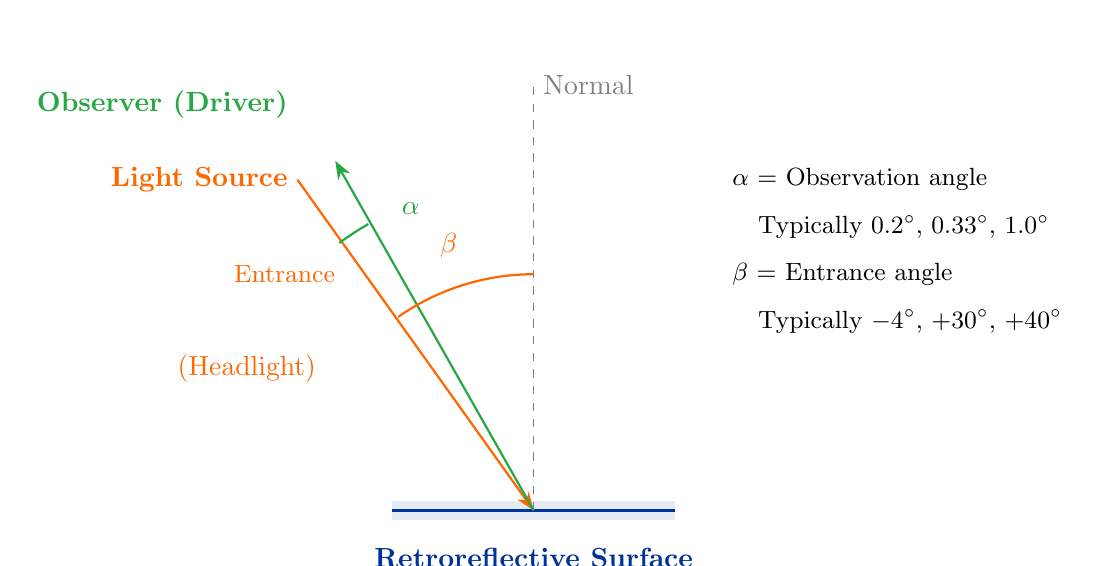
\begin{tikzpicture}[scale=1.2, >=Stealth]
    % Sign surface
    \fill[nhaiblue!10] (-1.5,-0.1) rectangle (1.5,0.1);
    \draw[thick, nhaiblue] (-1.5,0) -- (1.5,0);
    \node[below, nhaiblue] at (0,-0.3) {\textbf{Retroreflective Surface}};

    % Normal
    \draw[dashed, gray] (0,0) -- (0,4.5) node[right, gray] {Normal};

    % Entrance angle (light source)
    \draw[thick, nhaiorange, ->] (-2.5,3.5) -- (0,0);
    \node[nhaiorange, left] at (-2.5,3.5) {\textbf{Light Source}};
    \node[nhaiorange, left] at (-2.2,1.5) {(Headlight)};

    % Observation angle (observer)
    \draw[thick, successgreen, ->] (0,0) -- (-2.1,3.7);
    \node[successgreen, left] at (-2.5,4.3) {\textbf{Observer (Driver)}};

    % Entrance angle arc
    \draw[thick, nhaiorange] (0,2.5) arc (90:125:2.5);
    \node[nhaiorange] at (-0.9,2.8) {$\beta$};
    \node[nhaiorange, anchor=east] at (-2.0,2.5) {\small Entrance};

    % Observation angle arc (centered at origin, between observer ~120° and source ~126°)
    \draw[thick, successgreen] (120:3.5) arc (120:126:3.5);
    \node[successgreen] at (-1.3,3.2) {$\alpha$};

    % Annotations
    \node[right, font=\small] at (2, 3.5) {$\alpha$ = Observation angle};
    \node[right, font=\small] at (2, 3.0) {\quad Typically $0.2^{\circ}$, $0.33^{\circ}$, $1.0^{\circ}$};
    \node[right, font=\small] at (2, 2.5) {$\beta$ = Entrance angle};
    \node[right, font=\small] at (2, 2.0) {\quad Typically $-4^{\circ}$, $+30^{\circ}$, $+40^{\circ}$};
\end{tikzpicture}
\caption{Standard retroreflectivity measurement geometry showing entrance angle ($\beta$) and observation angle ($\alpha$). IRC~67 specifies measurements at $\alpha = 0.2^{\circ}$, $\beta = -4^{\circ}$ for traffic signs.}
\label{fig:measurement_geometry}
\end{figure}

\subsection{IRC Minimum Retroreflectivity Standards}

\begin{table}[H]
\centering
\caption{Minimum Retroreflectivity Requirements per IRC~67 (Signs) --- $R_A$ values in cd/lx/m$^2$}
\label{tab:irc67}
\begin{tabular}{@{}lcccc@{}}
\toprule
\textbf{Sheeting Type} & \textbf{White} & \textbf{Yellow} & \textbf{Red} & \textbf{Green} \\
\midrule
Type I (Engineering Grade) & 50 & 25 & 7 & 9 \\
Type III (High Intensity) & 120 & 65 & 20 & 21 \\
Type IV (Diamond Grade) & 250 & 170 & 45 & 45 \\
\bottomrule
\end{tabular}
\end{table}

\begin{table}[H]
\centering
\caption{Minimum Retroreflectivity Requirements per IRC~35 (Road Markings) --- $R_L$ values in mcd/lx/m$^2$}
\label{tab:irc35}
\begin{tabular}{@{}lcc@{}}
\toprule
\textbf{Marking Type} & \textbf{Dry Condition} & \textbf{Wet Condition} \\
\midrule
White Thermoplastic & 150 & 50 \\
Yellow Thermoplastic & 100 & 35 \\
Raised Pavement Markers (RPMs) & \multicolumn{2}{c}{Specific Intensity $\geq$ 5.0 cd/lux} \\
\bottomrule
\end{tabular}
\end{table}

\subsection{Degradation Mechanisms}

Retroreflective materials degrade through multiple mechanisms, each with characteristic time constants:

\begin{equation}
R_L(t) = R_L(0) \cdot \prod_{k=1}^{K} e^{-\lambda_k \cdot f_k(t)}
\label{eq:degradation_model}
\end{equation}

where $R_L(0)$ is the initial retroreflectivity, and $\lambda_k$ are degradation rate constants for each mechanism $k$:

\begin{table}[H]
\centering
\caption{Retroreflectivity Degradation Mechanisms and Factors}
\label{tab:degradation}
\begin{tabular}{@{}p{3cm}p{5cm}p{5cm}@{}}
\toprule
\textbf{Mechanism} & \textbf{Cause} & \textbf{Rate Factor $f_k(t)$} \\
\midrule
UV Degradation & Solar radiation breaks polymer bonds in sheeting & Cumulative solar exposure (kWh/m$^2$) \\
Abrasion & Vehicle tyre contact (markings), wind-borne particles (signs) & Cumulative AADT $\times$ lane distribution \\
Chemical Attack & Exhaust fumes, industrial pollution, de-icing salts & Cumulative pollutant concentration \\
Moisture Ingress & Rain, condensation penetrating sheeting layers & Wet-cycle count, humidity exposure \\
Thermal Cycling & Expansion/contraction causing microcracking & Temperature range $\times$ cycle count \\
Dirt Accumulation & Surface soiling reduces effective aperture & Time since last cleaning event \\
\bottomrule
\end{tabular}
\end{table}

\subsection{Existing Automated Measurement Technologies}

\begin{table}[H]
\centering
\caption{Comparison of Existing Retroreflectivity Measurement Approaches}
\label{tab:existing_tech}
\begin{tabular}{@{}p{3cm}p{2.5cm}p{2.5cm}p{2.5cm}p{2.5cm}@{}}
\toprule
\textbf{Technology} & \textbf{Speed} & \textbf{Cost} & \textbf{Accuracy} & \textbf{Limitation} \\
\midrule
Handheld (Delta LTL-X) & 2--5/hr & 5--10L per unit & $\pm$5\% & Dangerous, unscalable \\
Mobile (ECODYN) & 60 km/h & 1--2 Cr & $\pm$8\% & Signs only or markings only \\
LiDAR Survey & 80 km/h & 3--5 Cr & N/A & Measures geometry, not $R_L$ \\
\midrule
\textbf{RetroGuard (Ours)} & \textbf{Highway speed} & \textbf{Near-zero} & \textbf{Calibrated} & \textbf{Multi-modal} \\
\bottomrule
\end{tabular}
\end{table}


%==============================================================================
\section{RetroGuard System Architecture}
\label{sec:architecture}
%==============================================================================

The RetroGuard system is designed as a six-layer architecture where each layer independently delivers value, yet all layers synergistically feed into a unified Predictive Digital Twin. This design philosophy ensures that deployment can be incremental --- NHAI can begin with zero-cost layers (CCTV mining, smartphone app) and progressively activate additional layers.

\subsection{Architecture Overview}

\begin{figure}[H]
\centering
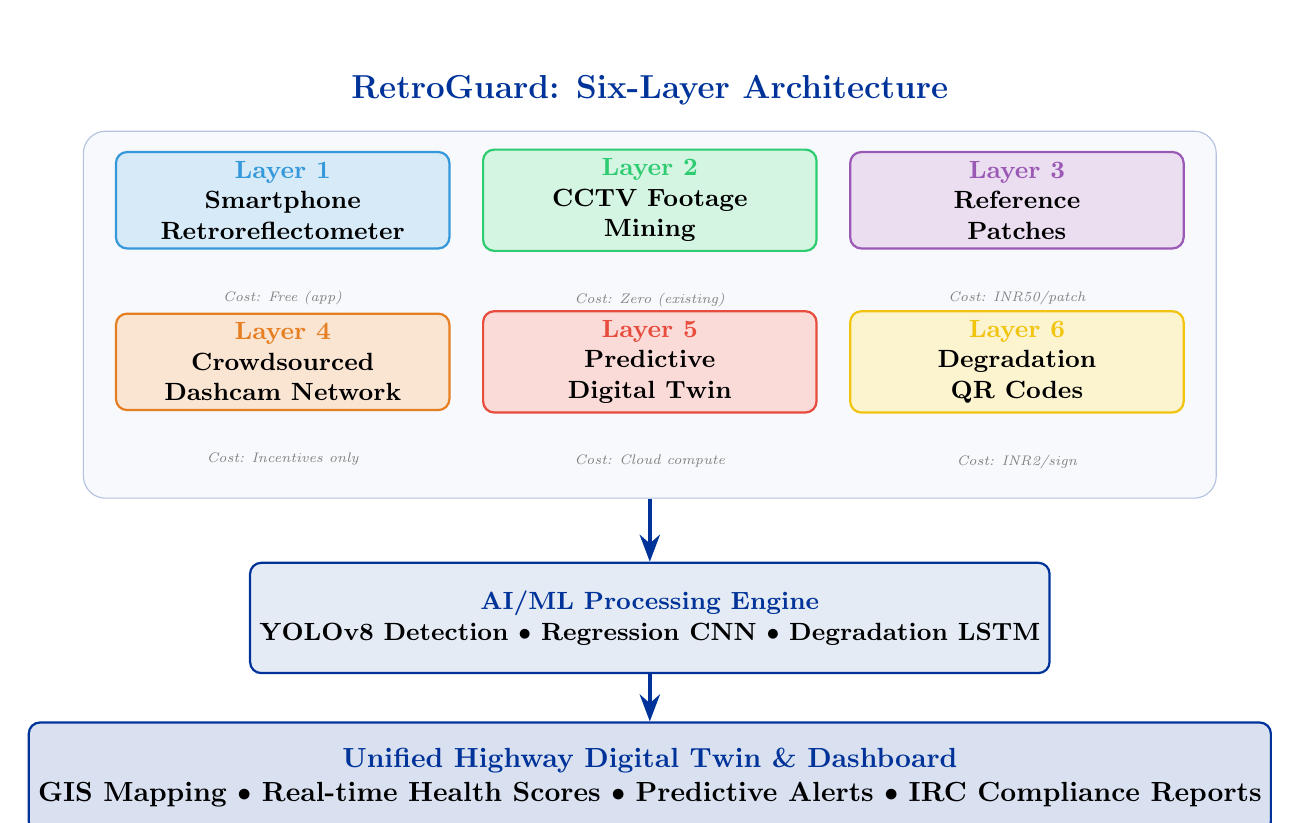
\begin{tikzpicture}[
    node distance=0.6cm and 0.8cm,
    layer/.style={rectangle, rounded corners=4pt, draw, thick, minimum width=4.2cm, minimum height=1.0cm, text width=4cm, align=center, font=\small\bfseries},
    aibox/.style={rectangle, rounded corners=4pt, draw=nhaiblue, thick, fill=nhaiblue!10, minimum width=10cm, minimum height=1.4cm, align=center, font=\small\bfseries},
    twinbox/.style={rectangle, rounded corners=4pt, draw=nhaiblue, thick, fill=nhaiblue!15, minimum width=12cm, minimum height=1.4cm, align=center, font=\bfseries},
    arrowstyle/.style={->, thick, >=Stealth},
    costlabel/.style={font=\tiny\itshape, text=codegray}
]

% Data Collection Layers (Top Row)
\node[layer, fill=layerA!20, draw=layerA] (L1) {\textcolor{layerA}{Layer 1}\\Smartphone\\Retroreflectometer};
\node[layer, fill=layerB!20, draw=layerB, right=0.4cm of L1] (L2) {\textcolor{layerB}{Layer 2}\\CCTV Footage\\Mining};
\node[layer, fill=layerC!20, draw=layerC, right=0.4cm of L2] (L3) {\textcolor{layerC}{Layer 3}\\Reference\\Patches};

% Cost labels (top row)
\node[costlabel, below=0.4cm of L1] (cost1) {Cost: Free (app)};
\node[costlabel, below=0.4cm of L2] (cost2) {Cost: Zero (existing)};
\node[costlabel, below=0.4cm of L3] (cost3) {Cost: \rupmark50/patch};

% Second Row
\node[layer, fill=layerD!20, draw=layerD, below=0.8cm of L1] (L4) {\textcolor{layerD}{Layer 4}\\Crowdsourced\\Dashcam Network};
\node[layer, fill=layerE!20, draw=layerE, right=0.4cm of L4] (L5) {\textcolor{layerE}{Layer 5}\\Predictive\\Digital Twin};
\node[layer, fill=layerF!20, draw=layerF, right=0.4cm of L5] (L6) {\textcolor{layerF}{Layer 6}\\Degradation\\QR Codes};

% Cost labels (bottom row)
\node[costlabel, below=0.4cm of L4] (cost4) {Cost: Incentives only};
\node[costlabel, below=0.4cm of L5] (cost5) {Cost: Cloud compute};
\node[costlabel, below=0.4cm of L6] (cost6) {Cost: \rupmark2/sign};

% Container grouping all data collection layers
\begin{pgfonlayer}{background}
\node[draw=nhaiblue!30, rounded corners=8pt, fill=nhaiblue!3,
      inner xsep=0.4cm, inner ysep=0.25cm,
      fit=(L1)(L3)(L4)(L6)(cost4)(cost5)(cost6)] (container) {};
\end{pgfonlayer}

% Title
\node[above=0.2cm of container.north, font=\large\bfseries\color{nhaiblue}] {RetroGuard: Six-Layer Architecture};

% AI Engine
\node[aibox, below=0.8cm of container] (AI) {\textcolor{nhaiblue}{AI/ML Processing Engine}\\YOLOv8 Detection $\bullet$ Regression CNN $\bullet$ Degradation LSTM};

% Digital Twin
\node[twinbox, below=0.6cm of AI] (DT) {\textcolor{nhaiblue}{Unified Highway Digital Twin \& Dashboard}\\GIS Mapping $\bullet$ Real-time Health Scores $\bullet$ Predictive Alerts $\bullet$ IRC Compliance Reports};

% Arrow from container to AI
\draw[arrowstyle, nhaiblue, line width=1.5pt] (container.south) -- (AI.north);

% Arrow from AI to DT
\draw[arrowstyle, nhaiblue, line width=1.5pt] (AI.south) -- (DT.north);

\end{tikzpicture}
\caption{RetroGuard system architecture. Six independent data collection layers feed into a unified AI/ML processing engine, which maintains a Predictive Highway Digital Twin. Each layer can be deployed independently, enabling incremental adoption.}
\label{fig:architecture}
\end{figure}

\subsection{Design Principles}

\begin{enumerate}[noitemsep]
    \item \textbf{Zero-Infrastructure-First:} Layers~1 and~2 require no new hardware purchase, only software deployment
    \item \textbf{Graceful Scaling:} Each additional layer improves coverage and accuracy without replacing previous layers
    \item \textbf{Calibration Independence:} Layer~3 (reference patches) provides universal calibration for all camera-based layers
    \item \textbf{Self-Improving:} The predictive model (Layer~5) improves as more data accumulates from all layers
    \item \textbf{Standards-Compliant:} All measurements are traceable to IRC~67/35 reference geometries through calibration
\end{enumerate}


%==============================================================================
\section{Layer 1: Smartphone Retroreflectometer}
\label{sec:layer1}
%==============================================================================

\subsection{Core Insight}

A smartphone contains two components that, combined, form the essential elements of a retroreflectometer:

\begin{itemize}[noitemsep]
    \item \textbf{Controlled Light Source:} LED flash with known spectral power distribution and luminous intensity
    \item \textbf{Calibrated Sensor:} CMOS camera sensor with known spectral response and linear intensity mapping (via RAW capture)
\end{itemize}

The key innovation is that by capturing images in RAW format (available on modern smartphones via Camera2 API / AVFoundation), we can obtain linear, radiometrically meaningful pixel values rather than gamma-corrected JPEG values.

\subsection{Mathematical Foundation}

The retroreflectivity coefficient can be estimated from smartphone measurements as:

\begin{equation}
\hat{R}_L = \frac{L_{measured}}{E_{\perp}} = \frac{K_{cam} \cdot \overline{P}_{target}}{I_{flash} \cdot \cos\beta / d^2}
\label{eq:smartphone_rl}
\end{equation}

where:
\begin{itemize}[noitemsep]
    \item $\overline{P}_{target}$ is the mean RAW pixel value of the target region
    \item $K_{cam}$ is the camera-to-luminance calibration constant (determined during calibration)
    \item $I_{flash}$ is the flash luminous intensity
    \item $\beta$ is the entrance angle
    \item $d$ is the distance from phone to target surface
\end{itemize}

\subsubsection{Calibration Protocol}

The calibration constant $K_{cam}$ is device-specific and determined using a \textbf{reference retroreflective patch} (a 10$\times$10 cm sample with factory-certified $R_L$ value):

\begin{equation}
K_{cam} = \frac{R_{L,ref} \cdot I_{flash} \cdot \cos\beta_{cal} / d_{cal}^2}{\overline{P}_{ref}}
\label{eq:calibration}
\end{equation}

Once calibrated, the phone can measure any retroreflective surface:

\begin{equation}
\hat{R}_{L,target} = R_{L,ref} \cdot \frac{\overline{P}_{target}}{\overline{P}_{ref}} \cdot \frac{d_{target}^2 \cdot \cos\beta_{ref}}{d_{ref}^2 \cdot \cos\beta_{target}}
\label{eq:ratio_measurement}
\end{equation}

This ratio-based formulation cancels out flash intensity variations, ambient light, and camera gain uncertainties.

\subsection{Measurement Protocol}

\begin{figure}[H]
\centering
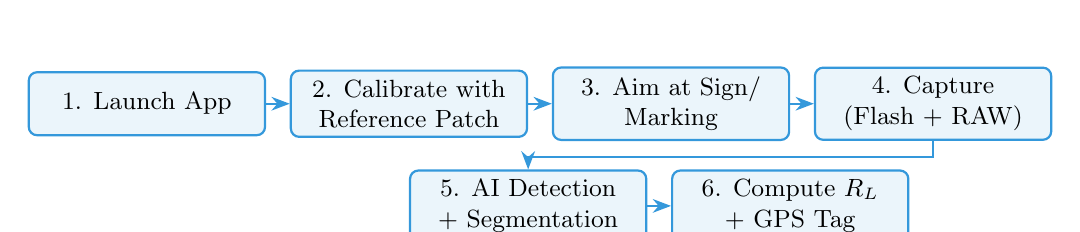
\begin{tikzpicture}[
    node distance=0.5cm,
    stepbox/.style={rectangle, rounded corners=3pt, draw=layerA, thick, fill=layerA!10, minimum width=3cm, minimum height=0.8cm, align=center, font=\small},
    arrowstyle/.style={->, thick, >=Stealth, layerA}
]
\node[stepbox] (S1) {1. Launch App};
\node[stepbox, right=0.3cm of S1] (S2) {2. Calibrate with\\Reference Patch};
\node[stepbox, right=0.3cm of S2] (S3) {3. Aim at Sign/\\Marking};
\node[stepbox, right=0.3cm of S3] (S4) {4. Capture\\(Flash + RAW)};
\node[stepbox, below=0.4cm of S2.south east] (S5) {5. AI Detection\\+ Segmentation};
\node[stepbox, right=0.3cm of S5] (S6) {6. Compute $R_L$\\+ GPS Tag};

\draw[arrowstyle] (S1) -- (S2);
\draw[arrowstyle] (S2) -- (S3);
\draw[arrowstyle] (S3) -- (S4);
\draw[arrowstyle] (S4.south) -- ++(0,-0.2) -| (S5.north);
\draw[arrowstyle] (S5) -- (S6);
\end{tikzpicture}
\caption{Smartphone retroreflectometer measurement workflow. Calibration (Step~2) is performed once per session using the reference patch.}
\label{fig:smartphone_workflow}
\end{figure}

\subsection{Error Analysis}

The measurement uncertainty propagation yields:

\begin{equation}
\frac{\sigma_{R_L}}{R_L} = \sqrt{\left(\frac{\sigma_P}{P}\right)^2 + 4\left(\frac{\sigma_d}{d}\right)^2 + \tan^2\beta \cdot \sigma_\beta^2}
\label{eq:error_propagation}
\end{equation}

For typical conditions (distance $d = 1.5 \pm 0.05$~m, angle $\beta = 4^{\circ} \pm 1^{\circ}$, pixel SNR $> 40$~dB):

\begin{equation}
\frac{\sigma_{R_L}}{R_L} \approx \sqrt{(0.01)^2 + 4(0.033)^2 + (0.0012)^2} \approx 6.8\%
\label{eq:error_estimate}
\end{equation}

This is comparable to the $\pm 5\%$ repeatability of commercial handheld retroreflectometers.

\subsection{Advantages Over Handheld Instruments}

\begin{table}[H]
\centering
\caption{Comparison: Smartphone App vs. Handheld Retroreflectometer}
\label{tab:smartphone_vs_handheld}
\begin{tabular}{@{}lcc@{}}
\toprule
\textbf{Parameter} & \textbf{Handheld (LTL-X)} & \textbf{RetroGuard App} \\
\midrule
Hardware Cost & 5--10 Lakh & Free (smartphone) \\
Calibration Device & 20,000 & 10 (reference sticker) \\
Training Required & 2--3 days & 10-minute in-app tutorial \\
Deployable Units & 10s (budget limited) & 10,000s (all inspectors) \\
GPS Tagging & Manual entry & Automatic \\
Photo Evidence & Separate camera & Integrated \\
Cloud Upload & Manual & Automatic \\
\bottomrule
\end{tabular}
\end{table}


%==============================================================================
\section{Layer 2: Existing CCTV Footage Mining}
\label{sec:layer2}
%==============================================================================

\subsection{Core Insight}

NHAI operates thousands of CCTV cameras along national highways for traffic monitoring and incident detection. Every night, vehicle headlights continuously illuminate road signs visible in these camera feeds. Each passing vehicle is an unintentional retroreflectivity test --- and this data is currently discarded.

\subsection{Physical Basis}

When a vehicle with headlights of luminous intensity $I_{headlight}$ passes at distance $d$ from a sign, the sign's apparent luminance in the CCTV image is:

\begin{equation}
L_{sign} = R_A \cdot \frac{I_{headlight} \cdot \cos\beta}{d_{sign-vehicle}^2}
\label{eq:cctv_luminance}
\end{equation}

The CCTV camera records pixel values proportional to this luminance:

\begin{equation}
P_{sign}(t) = K_{cctv} \cdot R_A \cdot \frac{I_{headlight}(t) \cdot \cos\beta(t)}{d(t)^2} + P_{ambient}(t) + n(t)
\label{eq:cctv_pixel}
\end{equation}

where $t$ indexes the time (vehicle passage), $P_{ambient}$ is background illumination, and $n(t)$ is sensor noise.

\subsection{Statistical Estimation from Multiple Vehicles}

The key insight is that while individual vehicle headlight intensity $I_{headlight}(t)$ is unknown, we observe \emph{hundreds} of vehicles per night passing the same sign. By analyzing the \textbf{distribution} of sign brightness across many vehicles, we can robustly estimate $R_A$:

\begin{equation}
\hat{R}_A = \frac{\text{median}_t\left[P_{sign}(t) - P_{ambient}(t)\right]}{K_{cctv} \cdot \overline{I}_{headlight} \cdot \overline{G}(\beta, d)}
\label{eq:cctv_estimation}
\end{equation}

where $\overline{I}_{headlight}$ is the expected headlight intensity for the Indian vehicle fleet (computed from beam pattern databases for Tata, Mahindra, Maruti, Ashok Leyland trucks, etc.), and $\overline{G}(\beta, d)$ is the average geometric factor.

\subsubsection{Vehicle Fleet Headlight Database}

We construct a headlight luminous intensity database for the Indian vehicle fleet:

\begin{table}[H]
\centering
\caption{Indian Vehicle Fleet Headlight Intensity Database (Low Beam)}
\label{tab:headlight_db}
\begin{tabular}{@{}lcc@{}}
\toprule
\textbf{Vehicle Category} & \textbf{Typical $I_{headlight}$ (cd)} & \textbf{Fleet Share (\%)} \\
\midrule
Passenger Car (Halogen) & 700--1,000 & 35 \\
Passenger Car (LED/HID) & 1,200--2,000 & 20 \\
SUV/MUV & 1,000--1,800 & 15 \\
LCV/Truck (Halogen) & 800--1,200 & 20 \\
Bus & 1,000--1,500 & 5 \\
Two-Wheeler & 200--500 & 5 \\
\bottomrule
\end{tabular}
\end{table}

\subsection{Temporal Trending}

The most powerful capability of CCTV mining is \textbf{automatic temporal trending}. By computing $\hat{R}_A$ nightly, we obtain a degradation curve without any manual intervention:

\begin{equation}
\hat{R}_A^{(night)} = \text{median}\left[\frac{P_{sign}(t_i) - P_{ambient}(t_i)}{G(t_i)}\right]_{i=1}^{N_{vehicles}}
\label{eq:nightly_ra}
\end{equation}

A sudden drop in nightly $\hat{R}_A$ may indicate:
\begin{itemize}[noitemsep]
    \item Physical damage to the sign (vandalism, vehicle impact)
    \item Dirt/dust accumulation (gradual decline, recoverable)
    \item Material degradation (monotonic decline, requires replacement)
\end{itemize}

\subsection{Processing Pipeline}

\begin{figure}[H]
\centering
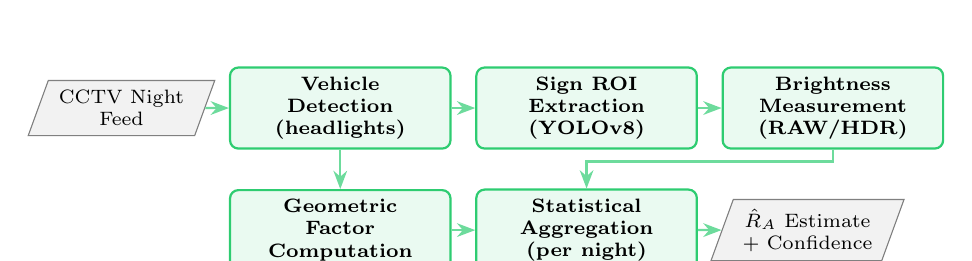
\begin{tikzpicture}[
    node distance=0.4cm,
    process/.style={rectangle, rounded corners=3pt, draw=layerB, thick, fill=layerB!10, minimum width=2.8cm, minimum height=1.0cm, align=center, font=\scriptsize\bfseries},
    data/.style={trapezium, trapezium left angle=70, trapezium right angle=110, draw=gray, fill=gray!10, minimum width=2cm, minimum height=0.7cm, align=center, font=\scriptsize},
    arrowstyle/.style={->, thick, >=Stealth, layerB!70}
]

\node[data] (input) {CCTV Night\\Feed};
\node[process, right=0.3cm of input] (detect) {Vehicle\\Detection\\(headlights)};
\node[process, right=0.3cm of detect] (sign) {Sign ROI\\Extraction\\(YOLOv8)};
\node[process, right=0.3cm of sign] (measure) {Brightness\\Measurement\\(RAW/HDR)};
\node[process, below=0.5cm of detect] (geo) {Geometric\\Factor\\Computation};
\node[process, right=0.3cm of geo] (stat) {Statistical\\Aggregation\\(per night)};
\node[data, right=0.3cm of stat] (output) {$\hat{R}_A$ Estimate\\+ Confidence};

\draw[arrowstyle] (input) -- (detect);
\draw[arrowstyle] (detect) -- (sign);
\draw[arrowstyle] (sign) -- (measure);
\draw[arrowstyle] (measure.south) -- ++(0,-0.15) -| (stat.north);
\draw[arrowstyle] (detect.south) -- (geo.north);
\draw[arrowstyle] (geo) -- (stat);
\draw[arrowstyle] (stat) -- (output);
\end{tikzpicture}
\caption{CCTV footage mining pipeline. Night-time frames are processed to extract sign brightness relative to headlight geometry, aggregated statistically across hundreds of vehicle passages per night.}
\label{fig:cctv_pipeline}
\end{figure}


%==============================================================================
\section{Layer 3: Retroreflective Reference Patches}
\label{sec:layer3}
%==============================================================================

\subsection{The Calibration Problem}

The fundamental challenge of camera-based retroreflectivity measurement is \textbf{calibration}: converting pixel brightness to absolute $R_L$ values. Camera exposure, gain, white balance, ambient light, and lens characteristics all affect the recorded brightness. Without calibration, measurements are meaningless.

\subsection{The Reference Patch Solution}

We propose installing small \textbf{retroreflective reference patches} with known, factory-certified retroreflectivity values near highway safety assets:

\begin{figure}[H]
\centering
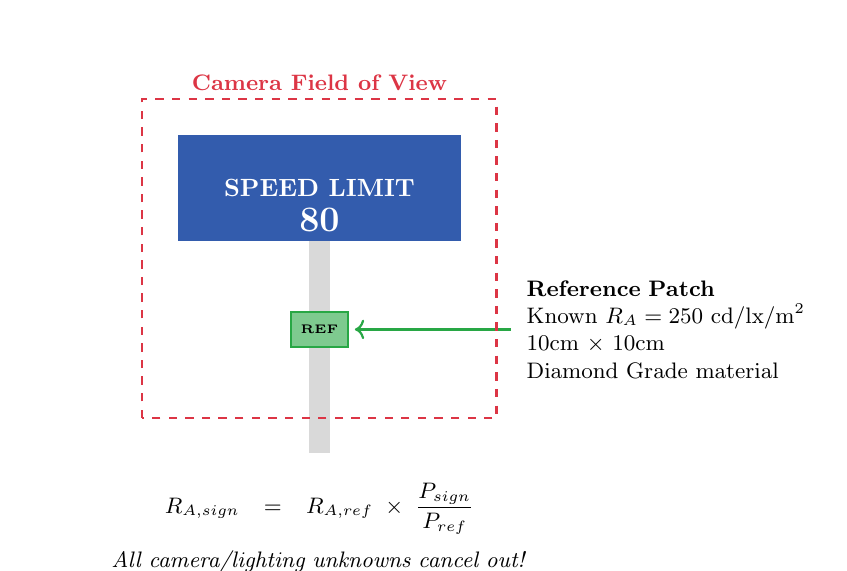
\begin{tikzpicture}[scale=0.9, transform shape]
    % Sign post
    \fill[gray!30] (-0.15, 0) rectangle (0.15, 3);

    % Sign
    \fill[nhaiblue!80] (-2.0, 3) rectangle (2.0, 4.5);
    \node[white, font=\bfseries] at (0, 3.75) {SPEED LIMIT};
    \node[white, font=\Large\bfseries] at (0, 3.3) {80};

    % Reference patch (on post)
    \fill[successgreen!60] (-0.4, 1.5) rectangle (0.4, 2.0);
    \draw[thick, successgreen] (-0.4, 1.5) rectangle (0.4, 2.0);
    \node[font=\tiny\bfseries] at (0, 1.75) {REF};

    % Arrow to patch
    \draw[->, thick, successgreen] (2.7, 1.75) -- (0.5, 1.75);
    \node[anchor=west, font=\small, text width=4cm] at (2.8, 1.75) {\textbf{Reference Patch}\\Known $R_A = 250$ cd/lx/m$^2$\\10cm $\times$ 10cm\\Diamond Grade material};

    % Camera view box
    \draw[dashed, criticalred, thick] (-2.5, 0.5) rectangle (2.5, 5.0);
    \node[criticalred, font=\small\bfseries, above] at (0, 5.0) {Camera Field of View};

    % Equation
    \node[below, font=\small, text width=8cm, align=center] at (0, -0.3) {
        $R_{A,sign} = R_{A,ref} \times \dfrac{P_{sign}}{P_{ref}}$ \\[0.2cm]
        \textit{All camera/lighting unknowns cancel out!}
    };
\end{tikzpicture}
\caption{Reference patch placement concept. The patch is visible in the same camera frame as the sign, enabling ratio-based measurement that cancels all environmental and camera variables.}
\label{fig:reference_patch}
\end{figure}

\subsection{Mathematical Cancellation}

When the reference patch and target sign are in the same camera frame, illuminated by the same light source:

\begin{equation}
\frac{P_{sign}}{P_{ref}} = \frac{K_{cam} \cdot R_{A,sign} \cdot E_{sign}}{K_{cam} \cdot R_{A,ref} \cdot E_{ref}}
\label{eq:ratio_cancel}
\end{equation}

If the patch is close to the sign (similar illumination geometry, $E_{sign} \approx E_{ref}$):

\begin{equation}
R_{A,sign} = R_{A,ref} \cdot \frac{P_{sign}}{P_{ref}} \cdot \underbrace{\frac{E_{ref}}{E_{sign}}}_{\approx 1 \text{ if co-located}}
\label{eq:patch_measurement}
\end{equation}

This eliminates dependence on:
\begin{itemize}[noitemsep]
    \item Camera type, exposure, gain, white balance
    \item Light source intensity and spectrum
    \item Ambient illumination conditions
    \item Distance to the measurement
    \item Atmospheric conditions (fog, rain)
\end{itemize}

\subsection{Patch Specifications}

\begin{table}[H]
\centering
\caption{Reference Patch Design Specifications}
\label{tab:patch_specs}
\begin{tabular}{@{}ll@{}}
\toprule
\textbf{Parameter} & \textbf{Specification} \\
\midrule
Material & Type IV (Diamond Grade) microprismatic sheeting \\
Size & 10 cm $\times$ 10 cm (sign-mounted) / 20 cm $\times$ 20 cm (pavement) \\
Certified $R_A$ & 300 $\pm$ 5 cd/lx/m$^2$ (white) \\
Service Life & $>$12 years (highest grade material, minimal wear) \\
Cost per Unit & $\sim$\rupmark50 \\
Placement & On sign post 1m below sign; on road shoulder near marking zones \\
QR Identifier & Unique ID linking to calibration certificate in cloud database \\
\bottomrule
\end{tabular}
\end{table}

\subsection{Impact on Other Layers}

Reference patches serve as a \textbf{universal calibration backbone} for the entire RetroGuard system:

\begin{itemize}[noitemsep]
    \item \textbf{Layer 1 (Smartphone):} Used as calibration target during measurement sessions
    \item \textbf{Layer 2 (CCTV):} Visible in CCTV frames, provides absolute calibration for CCTV-based estimates
    \item \textbf{Layer 4 (Dashcam):} Enables calibrated measurements from uncalibrated dashcams
    \item \textbf{Layer 5 (Digital Twin):} Provides ground-truth anchoring for ML model training
\end{itemize}


%==============================================================================
\section{Layer 4: Crowdsourced Dashcam Intelligence Network}
\label{sec:layer4}
%==============================================================================

\subsection{Scale of Opportunity}

India's national highways carry an estimated 1.5 million commercial vehicles daily. An increasing fraction are equipped with dashcams (mandatory for fleet insurance in many cases). This represents an enormous, untapped measurement fleet.

\subsection{System Design}

\begin{figure}[H]
\centering
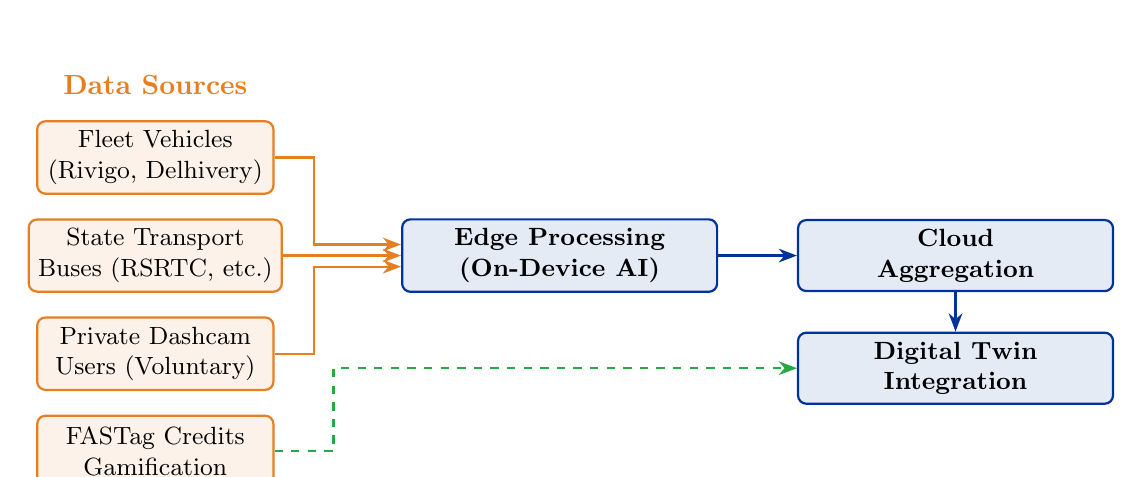
\begin{tikzpicture}[
    node distance=0.5cm,
    box/.style={rectangle, rounded corners=3pt, draw=layerD, thick, fill=layerD!10, minimum width=3.0cm, minimum height=0.9cm, align=center, font=\small},
    cloudbox/.style={rectangle, rounded corners=3pt, draw=nhaiblue, thick, fill=nhaiblue!10, minimum width=4.0cm, minimum height=0.9cm, align=center, font=\small\bfseries},
    arrowstyle/.style={->, thick, >=Stealth}
]

% Data sources
\node[box] (fleet) {Fleet Vehicles\\(Rivigo, Delhivery)};
\node[box, below=0.3cm of fleet] (bus) {State Transport\\Buses (RSRTC, etc.)};
\node[box, below=0.3cm of bus] (private) {Private Dashcam\\Users (Voluntary)};

% Processing
\node[cloudbox, right=1.5cm of bus] (edge) {Edge Processing\\(On-Device AI)};
\node[cloudbox, right=1.0cm of edge] (cloud) {Cloud\\Aggregation};
\node[cloudbox, below=0.5cm of cloud] (twin) {Digital Twin\\Integration};

% Incentives
\node[box, below=0.3cm of private] (reward) {FASTag Credits\\Gamification};

\draw[arrowstyle, layerD] (fleet.east) -- ++(0.5,0) |- ([yshift=4pt]edge.west);
\draw[arrowstyle, layerD] (bus.east) -- (edge.west);
\draw[arrowstyle, layerD] (private.east) -- ++(0.5,0) |- ([yshift=-4pt]edge.west);
\draw[arrowstyle, nhaiblue] (edge) -- (cloud);
\draw[arrowstyle, nhaiblue] (cloud) -- (twin);
\draw[arrowstyle, successgreen, dashed] (reward.east) -- ++(0.75,0) |- (twin.west);

\node[above=0.2cm of fleet, font=\bfseries\color{layerD}] {Data Sources};
\end{tikzpicture}
\caption{Crowdsourced dashcam network architecture. On-device AI processes footage locally, transmitting only metadata (sign location, brightness measurement, GPS) to minimize bandwidth.}
\label{fig:crowdsource}
\end{figure}

\subsection{Edge Processing for Privacy and Bandwidth}

Rather than uploading raw video, the RetroGuard SDK processes footage \textbf{on-device}:

\begin{enumerate}[noitemsep]
    \item \textbf{Detect} signs/markings in dashcam frame (lightweight YOLOv8-nano, $<$10ms on mobile GPU)
    \item \textbf{Extract} brightness metadata from detected regions
    \item \textbf{Compute} geometric factors from vehicle speed + GPS
    \item \textbf{Transmit} only: GPS coordinates, timestamp, asset type, brightness value, confidence score ($\sim$200 bytes per observation)
\end{enumerate}

This approach:
\begin{itemize}[noitemsep]
    \item Preserves driver privacy (no video leaves the device)
    \item Requires $<$1 KB/observation bandwidth
    \item Enables real-time processing even with intermittent connectivity
\end{itemize}

\subsection{Coverage Estimation}

For a highway segment with Average Annual Daily Traffic (AADT) of $N$ vehicles, and dashcam penetration rate $p$:

\begin{equation}
n_{observations/day} = N \cdot p \cdot P_{detect}
\label{eq:coverage}
\end{equation}

where $P_{detect}$ is the probability of successful detection per passage. With conservative estimates ($N = 10,000$, $p = 5\%$, $P_{detect} = 0.3$ at night):

\begin{equation}
n_{observations/day} = 10{,}000 \times 0.05 \times 0.3 = 150 \text{ observations/day}
\label{eq:coverage_est}
\end{equation}

This provides statistically robust measurements for every sign along the highway.


%==============================================================================
\section{Layer 5: Predictive Digital Twin}
\label{sec:layer5}
%==============================================================================

\subsection{Concept}

The Predictive Digital Twin is a GIS-based platform where every retroreflective asset on the national highway network exists as a digital entity with continuously updated health status and predicted remaining service life.

\subsection{Asset Data Model}

Each highway safety asset is represented as:

\begin{equation}
\mathcal{A}_i = \left\{id_i, \text{type}_i, \text{loc}_i, t_{install}, \text{material}_i, R_L^{(history)}, \hat{R}_L^{(predicted)}, \text{confidence}_i\right\}
\label{eq:asset_model}
\end{equation}

\subsection{ML Degradation Prediction}

We employ an LSTM-based time series model for retroreflectivity degradation prediction:

\begin{equation}
\hat{R}_L(t + \Delta t) = f_{LSTM}\left(R_L^{(t-T:t)}, \mathbf{X}_{env}^{(t-T:t)}, \mathbf{X}_{traffic}^{(t-T:t)}\right)
\label{eq:lstm_prediction}
\end{equation}

where:
\begin{itemize}[noitemsep]
    \item $R_L^{(t-T:t)}$ is the historical retroreflectivity sequence over window $T$
    \item $\mathbf{X}_{env}$ includes environmental covariates: temperature, rainfall, humidity, UV index, pollution (PM2.5) from IMD/CPCB APIs
    \item $\mathbf{X}_{traffic}$ includes traffic data: AADT, heavy vehicle percentage, lane distribution from NHAI ATMS
\end{itemize}

\subsubsection{Feature Engineering}

\begin{table}[H]
\centering
\caption{Predictive Model Feature Set}
\label{tab:features}
\begin{tabular}{@{}llp{6cm}@{}}
\toprule
\textbf{Category} & \textbf{Feature} & \textbf{Source} \\
\midrule
\multirow{3}{*}{Asset} & Material type/grade & Installation records \\
 & Age since installation & Installation date \\
 & Orientation (N/S/E/W) & GIS coordinates \\
\midrule
\multirow{4}{*}{Environmental} & Cumulative rainfall & IMD API \\
 & Temperature range & IMD API \\
 & UV exposure index & Solar radiation data \\
 & PM2.5 concentration & CPCB API \\
\midrule
\multirow{3}{*}{Traffic} & AADT & NHAI ATMS \\
 & Heavy vehicle \% & NHAI toll data \\
 & Speed profile & NHAI ATMS \\
\midrule
\multirow{2}{*}{Historical} & $R_L$ time series & RetroGuard measurements \\
 & Degradation rate & Computed from time series \\
\bottomrule
\end{tabular}
\end{table}

\subsection{Maintenance Optimization}

The Digital Twin enables a shift from time-based to \textbf{condition-based predictive maintenance}:

\begin{equation}
t_{replacement} = \min\left\{t : \hat{R}_L(t) < R_{L,min}^{IRC}\right\}
\label{eq:replacement_time}
\end{equation}

The system generates prioritized maintenance work orders:

\begin{equation}
\text{Priority}_i = w_1 \cdot \frac{R_{L,min} - \hat{R}_L(t_{now})}{R_{L,min}} + w_2 \cdot \text{AADT}_i + w_3 \cdot \text{Accident\_History}_i
\label{eq:priority}
\end{equation}

where $w_1, w_2, w_3$ are configurable weights balancing retroreflectivity deficit, traffic exposure, and safety history.

\subsection{Dashboard Design}

\begin{figure}[H]
\centering
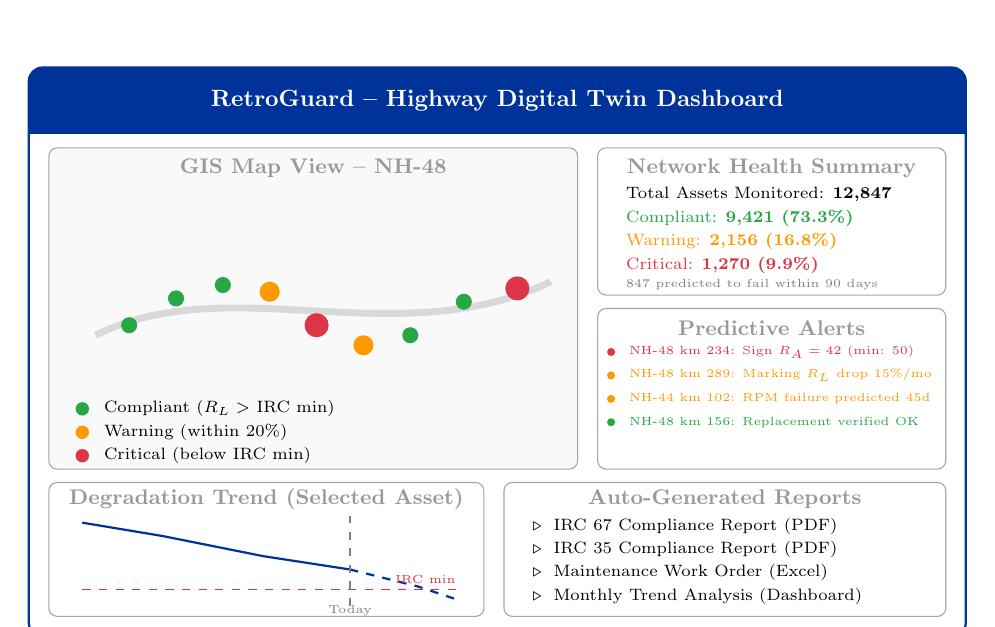
\begin{tikzpicture}[scale=0.85, transform shape]
    % Dashboard background
    \fill[white, rounded corners=5pt] (0,0) rectangle (14, 8.5);

    % Main dashboard frame
    \draw[thick, nhaiblue, rounded corners=5pt] (0,0) rectangle (14, 8.5);

    % Title bar (clipped to match rounded frame)
    \begin{scope}
        \clip[rounded corners=5pt] (0,0) rectangle (14, 8.5);
        \fill[nhaiblue] (0, 7.5) rectangle (14, 8.6);
    \end{scope}
    \node[white, font=\bfseries] at (7, 8.0) {RetroGuard -- Highway Digital Twin Dashboard};

    % ==== GIS Map Panel ====
    \fill[gray!5, rounded corners=3pt] (0.3, 2.5) rectangle (8.2, 7.3);
    \draw[gray!70, rounded corners=3pt] (0.3, 2.5) rectangle (8.2, 7.3);
    \node[font=\small\bfseries, gray!80] at (4.25, 7.0) {GIS Map View -- NH-48};

    % Highway line (drawn before dots so dots sit on top)
    \draw[gray!30, line width=2.5pt] (1.0, 4.5) .. controls (3, 5.5) and (5.5, 4.2) .. (7.8, 5.3);

    % Map dots along highway
    \fill[successgreen] (1.5, 4.65) circle (0.12);
    \fill[successgreen] (2.2, 5.05) circle (0.12);
    \fill[successgreen] (2.9, 5.25) circle (0.12);
    \fill[warningorange] (3.6, 5.15) circle (0.15);
    \fill[criticalred] (4.3, 4.65) circle (0.18);
    \fill[warningorange] (5.0, 4.35) circle (0.15);
    \fill[successgreen] (5.7, 4.5) circle (0.12);
    \fill[successgreen] (6.5, 5.0) circle (0.12);
    \fill[criticalred] (7.3, 5.2) circle (0.18);

    % Legend
    \fill[successgreen] (0.8, 3.4) circle (0.1);
    \node[right, font=\scriptsize] at (1.0, 3.4) {Compliant ($R_L >$ IRC min)};
    \fill[warningorange] (0.8, 3.05) circle (0.1);
    \node[right, font=\scriptsize] at (1.0, 3.05) {Warning (within 20\%)};
    \fill[criticalred] (0.8, 2.7) circle (0.1);
    \node[right, font=\scriptsize] at (1.0, 2.7) {Critical (below IRC min)};

    % ==== Network Health Summary Panel ====
    \draw[gray!70, rounded corners=3pt] (8.5, 5.1) rectangle (13.7, 7.3);
    \node[font=\small\bfseries, gray!80] at (11.1, 7.0) {Network Health Summary};
    \node[font=\scriptsize, anchor=west] at (8.8, 6.6) {Total Assets Monitored: \textbf{12,847}};
    \node[font=\scriptsize, successgreen, anchor=west] at (8.8, 6.25) {Compliant: \textbf{9,421 (73.3\%)}};
    \node[font=\scriptsize, warningorange, anchor=west] at (8.8, 5.9) {Warning: \textbf{2,156 (16.8\%)}};
    \node[font=\scriptsize, criticalred, anchor=west] at (8.8, 5.55) {Critical: \textbf{1,270 (9.9\%)}};
    \node[font=\tiny, gray, anchor=west] at (8.8, 5.25) {847 predicted to fail within 90 days};

    % ==== Predictive Alerts Panel ====
    \draw[gray!70, rounded corners=3pt] (8.5, 2.5) rectangle (13.7, 4.9);
    \node[font=\small\bfseries, gray!80] at (11.1, 4.6) {Predictive Alerts};
    \fill[criticalred] (8.7, 4.25) circle (0.06);
    \node[font=\tiny, criticalred, anchor=west] at (8.85, 4.25) {NH-48 km 234: Sign $R_A = 42$ (min: 50)};
    \fill[warningorange] (8.7, 3.9) circle (0.06);
    \node[font=\tiny, warningorange, anchor=west] at (8.85, 3.9) {NH-48 km 289: Marking $R_L$ drop 15\%/mo};
    \fill[warningorange] (8.7, 3.55) circle (0.06);
    \node[font=\tiny, warningorange, anchor=west] at (8.85, 3.55) {NH-44 km 102: RPM failure predicted 45d};
    \fill[successgreen] (8.7, 3.2) circle (0.06);
    \node[font=\tiny, successgreen, anchor=west] at (8.85, 3.2) {NH-48 km 156: Replacement verified OK};

    % ==== Degradation Trend Panel ====
    \draw[gray!70, rounded corners=3pt] (0.3, 0.3) rectangle (6.8, 2.3);
    \node[font=\small\bfseries, gray!80] at (3.55, 2.05) {Degradation Trend (Selected Asset)};
    % Measured data (solid)
    \draw[thick, nhaiblue] (0.8, 1.7) -- (2.0, 1.5) -- (3.5, 1.2) -- (4.8, 1.0);
    % Predicted data (dashed)
    \draw[thick, nhaiblue, dashed] (4.8, 1.0) -- (5.8, 0.75) -- (6.4, 0.55);
    % IRC minimum threshold
    \draw[dashed, criticalred] (0.8, 0.7) -- (6.5, 0.7);
    \node[font=\tiny, criticalred, anchor=east] at (6.5, 0.85) {IRC min};
    % Today marker
    \draw[dashed, gray] (4.8, 0.45) -- (4.8, 1.8);
    \node[font=\tiny, gray] at (4.8, 0.38) {Today};

    % ==== Auto-Generated Reports Panel ====
    \draw[gray!70, rounded corners=3pt] (7.1, 0.3) rectangle (13.7, 2.3);
    \node[font=\small\bfseries, gray!80] at (10.4, 2.05) {Auto-Generated Reports};
    \node[font=\scriptsize, anchor=west] at (7.4, 1.65) {$\triangleright$\; IRC~67 Compliance Report (PDF)};
    \node[font=\scriptsize, anchor=west] at (7.4, 1.3) {$\triangleright$\; IRC~35 Compliance Report (PDF)};
    \node[font=\scriptsize, anchor=west] at (7.4, 0.95) {$\triangleright$\; Maintenance Work Order (Excel)};
    \node[font=\scriptsize, anchor=west] at (7.4, 0.6) {$\triangleright$\; Monthly Trend Analysis (Dashboard)};
\end{tikzpicture}
\caption{RetroGuard Digital Twin Dashboard mockup showing GIS map with asset health status, predictive alerts, degradation trending, and automated compliance reporting.}
\label{fig:dashboard}
\end{figure}


%==============================================================================
\section{Layer 6: Degradation-Encoding QR Codes}
\label{sec:layer6}
%==============================================================================

\subsection{Self-Reporting Signs}

The most innovative layer of RetroGuard encodes retroreflectivity health information directly into the sign itself during manufacturing.

\subsection{Design Principle}

A QR code is printed on the sign using the \textbf{same retroreflective sheeting material} as the sign face. Since the QR code and the sign face share identical material, they degrade at the same rate. The readability of the QR code directly indicates the retroreflective health of the sign:

\begin{figure}[H]
\centering
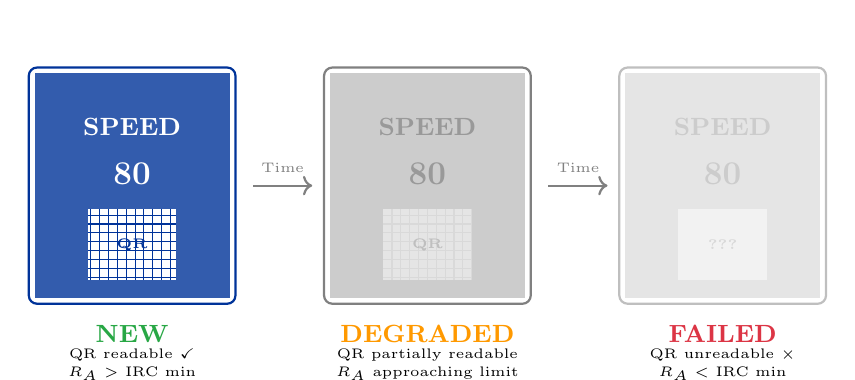
\begin{tikzpicture}[scale=0.75]
    % New sign
    \draw[thick, nhaiblue, rounded corners=3pt] (0,0) rectangle (3.5, 4);
    \fill[nhaiblue!80] (0.1,0.1) rectangle (3.4, 3.9);
    \node[white, font=\bfseries\small] at (1.75, 3.0) {SPEED};
    \node[white, font=\bfseries\large] at (1.75, 2.2) {80};
    % QR placeholder
    \fill[white] (1.0, 0.4) rectangle (2.5, 1.6);
    \draw[nhaiblue, thin, xstep=0.15cm, ystep=0.15cm] (1.0, 0.4) grid (2.5, 1.6);
    \node[font=\tiny\bfseries, nhaiblue] at (1.75, 1.0) {QR};

    \node[below, font=\small\bfseries, successgreen] at (1.75, -0.2) {NEW};
    \node[below, font=\tiny] at (1.75, -0.6) {QR readable $\checkmark$};
    \node[below, font=\tiny] at (1.75, -0.9) {$R_A > $ IRC min};

    % Degraded sign
    \draw[thick, gray, rounded corners=3pt] (5,0) rectangle (8.5, 4);
    \fill[gray!40] (5.1,0.1) rectangle (8.4, 3.9);
    \node[gray!80, font=\bfseries\small] at (6.75, 3.0) {SPEED};
    \node[gray!80, font=\bfseries\large] at (6.75, 2.2) {80};
    % Degraded QR
    \fill[gray!20] (6.0, 0.4) rectangle (7.5, 1.6);
    \draw[gray!30, thin, xstep=0.15cm, ystep=0.15cm] (6.0, 0.4) grid (7.5, 1.6);
    \node[font=\tiny\bfseries, gray!50] at (6.75, 1.0) {QR};

    \node[below, font=\small\bfseries, warningorange] at (6.75, -0.2) {DEGRADED};
    \node[below, font=\tiny] at (6.75, -0.6) {QR partially readable};
    \node[below, font=\tiny] at (6.75, -0.9) {$R_A$ approaching limit};

    % Failed sign
    \draw[thick, gray!50, rounded corners=3pt] (10,0) rectangle (13.5, 4);
    \fill[gray!20] (10.1,0.1) rectangle (13.4, 3.9);
    \node[gray!40, font=\bfseries\small] at (11.75, 3.0) {SPEED};
    \node[gray!40, font=\bfseries\large] at (11.75, 2.2) {80};
    % Unreadable QR
    \fill[gray!10] (11.0, 0.4) rectangle (12.5, 1.6);
    \node[font=\tiny\bfseries, gray!30] at (11.75, 1.0) {???};

    \node[below, font=\small\bfseries, criticalred] at (11.75, -0.2) {FAILED};
    \node[below, font=\tiny] at (11.75, -0.6) {QR unreadable $\times$};
    \node[below, font=\tiny] at (11.75, -0.9) {$R_A < $ IRC min};

    % Arrow timeline
    \draw[->, thick, gray] (3.8, 2) -- (4.8, 2);
    \draw[->, thick, gray] (8.8, 2) -- (9.8, 2);
    \node[font=\tiny, gray] at (4.3, 2.3) {Time};
    \node[font=\tiny, gray] at (9.3, 2.3) {Time};
\end{tikzpicture}
\caption{Degradation-encoding QR code concept. The QR code, made from the same retroreflective material as the sign, degrades identically. QR readability serves as a binary proxy for retroreflective health.}
\label{fig:qr_degradation}
\end{figure}

\subsection{QR Code Encoded Data}

Each QR code encodes:

\begin{table}[H]
\centering
\caption{QR Code Data Fields}
\label{tab:qr_data}
\begin{tabular}{@{}lll@{}}
\toprule
\textbf{Field} & \textbf{Size} & \textbf{Purpose} \\
\midrule
Asset UUID & 16 bytes & Unique identifier linking to Digital Twin \\
Installation Date & 4 bytes & Age computation \\
Material Grade & 1 byte & IRC threshold lookup \\
$R_{A,initial}$ & 2 bytes & Baseline retroreflectivity \\
GPS Coordinates & 8 bytes & Location verification \\
Highway ID & 4 bytes & Network identification \\
Manufacturer ID & 2 bytes & Quality tracking / warranty \\
\midrule
\textbf{Total} & \textbf{37 bytes} & Version~2 QR (25$\times$25 modules) sufficient \\
\bottomrule
\end{tabular}
\end{table}

\subsection{Error Correction as Degradation Proxy}

QR codes use Reed-Solomon error correction with four levels (L/M/Q/H). By designing at Level~H (30\% error correction), we create a \textbf{graduated degradation indicator}:

\begin{equation}
\text{Health Estimate} = \begin{cases}
\text{Compliant} & \text{if decoded at Level L (7\% correction)} \\
\text{Warning} & \text{if decoded at Level M (15\%) but not L} \\
\text{Critical} & \text{if decoded at Level H (30\%) but not M} \\
\text{Failed} & \text{if not decodable at Level H}
\end{cases}
\label{eq:qr_health}
\end{equation}

\subsection{Manufacturing Integration}

The QR code can be integrated into sign manufacturing at negligible marginal cost ($\sim$\rupmark2 per sign):
\begin{itemize}[noitemsep]
    \item Printed during sheeting application using the same material
    \item No additional manufacturing step --- just a pattern in the retroreflective layer
    \item NHAI can mandate this in procurement specifications for all new signs
\end{itemize}


%==============================================================================
\section{AI/ML Processing Pipeline}
\label{sec:ai_pipeline}
%==============================================================================

\subsection{Object Detection: Sign and Marking Recognition}

The detection pipeline must identify retroreflective assets across diverse conditions (day/night, dry/wet, fog).

\subsubsection{Model Architecture}

We employ a two-stage approach:

\begin{enumerate}[noitemsep]
    \item \textbf{Primary Detector:} YOLOv8-Large for real-time detection at highway speeds
    \item \textbf{Verification Detector:} RT-DETR (Real-Time Detection Transformer) for high-confidence verification of critical detections
\end{enumerate}

The YOLOv8 loss function combines three components:

\begin{equation}
\mathcal{L}_{total} = \lambda_{box} \cdot \mathcal{L}_{CIoU} + \lambda_{cls} \cdot \mathcal{L}_{BCE} + \lambda_{dfl} \cdot \mathcal{L}_{DFL}
\label{eq:yolo_loss}
\end{equation}

where:
\begin{itemize}[noitemsep]
    \item $\mathcal{L}_{CIoU}$ is the Complete IoU loss for bounding box regression
    \item $\mathcal{L}_{BCE}$ is Binary Cross-Entropy for classification
    \item $\mathcal{L}_{DFL}$ is Distribution Focal Loss for precise localization
\end{itemize}

\subsubsection{Detection Classes}

\begin{table}[H]
\centering
\caption{RetroGuard Object Detection Classes}
\label{tab:classes}
\begin{tabular}{@{}clc@{}}
\toprule
\textbf{Class ID} & \textbf{Asset Type} & \textbf{IRC Standard} \\
\midrule
0 & Regulatory Sign (speed limit, stop, yield) & IRC~67 \\
1 & Warning Sign (curve, intersection, hazard) & IRC~67 \\
2 & Informatory Sign (destination, distance) & IRC~67 \\
3 & Gantry-Mounted Sign & IRC~67 \\
4 & White Pavement Marking (lane, edge) & IRC~35 \\
5 & Yellow Pavement Marking (median, no-passing) & IRC~35 \\
6 & Raised Pavement Marker (RPM/road stud) & IRC~35 \\
7 & Delineator Post & IRC~35 \\
8 & Reference Calibration Patch & Internal \\
\bottomrule
\end{tabular}
\end{table}

\subsection{Retroreflectivity Estimation CNN}

After detection, a specialized regression CNN estimates the retroreflectivity coefficient from the cropped image patch.

\subsubsection{Architecture}

\begin{figure}[H]
\centering
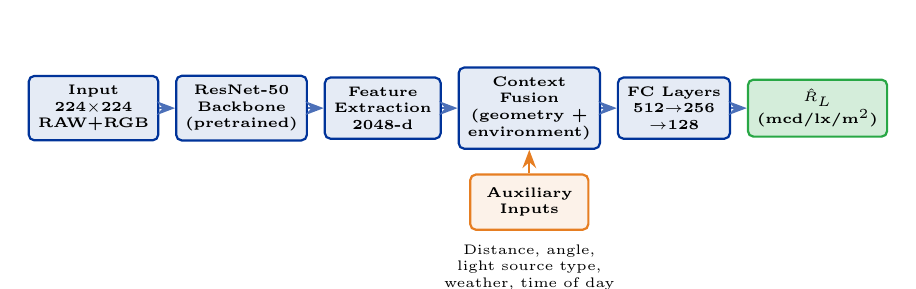
\begin{tikzpicture}[
    node distance=0.3cm,
    block/.style={rectangle, rounded corners=2pt, draw=nhaiblue, thick, fill=nhaiblue!10, minimum height=0.7cm, align=center, font=\tiny\bfseries},
    arrowstyle/.style={->, thick, >=Stealth, nhaiblue!70}
]

\node[block, minimum width=1.2cm] (input) {Input\\224$\times$224\\RAW+RGB};
\node[block, right=0.2cm of input, minimum width=1.2cm] (enc) {ResNet-50\\Backbone\\(pretrained)};
\node[block, right=0.2cm of enc, minimum width=1.2cm] (feat) {Feature\\Extraction\\2048-d};
\node[block, right=0.2cm of feat, minimum width=1.5cm] (context) {Context\\Fusion\\(geometry +\\environment)};
\node[block, right=0.2cm of context, minimum width=1.2cm] (fc) {FC Layers\\512$\to$256\\$\to$128};
\node[block, right=0.2cm of fc, minimum width=1.2cm, fill=successgreen!20, draw=successgreen] (output) {$\hat{R}_L$\\(mcd/lx/m$^2$)};

\draw[arrowstyle] (input) -- (enc);
\draw[arrowstyle] (enc) -- (feat);
\draw[arrowstyle] (feat) -- (context);
\draw[arrowstyle] (context) -- (fc);
\draw[arrowstyle] (fc) -- (output);

% Context inputs
\node[block, below=0.3cm of context, minimum width=1.5cm, fill=layerD!10, draw=layerD] (aux) {Auxiliary\\Inputs};
\draw[arrowstyle, layerD] (aux) -- (context);
\node[font=\tiny, below=0.05cm of aux, text width=3cm, align=center] {Distance, angle,\\light source type,\\weather, time of day};

\end{tikzpicture}
\caption{Retroreflectivity estimation CNN architecture. A ResNet-50 backbone extracts visual features, which are fused with geometric and environmental context before regression to $R_L$.}
\label{fig:cnn_architecture}
\end{figure}

\subsubsection{Loss Function}

We use a composite loss combining Mean Squared Error with a threshold-aware penalty:

\begin{equation}
\mathcal{L}_{retro} = \frac{1}{N}\sum_{i=1}^{N}\left[\left(\hat{R}_{L,i} - R_{L,i}\right)^2 + \lambda \cdot \max\left(0, R_{L,min} - \hat{R}_{L,i}\right) \cdot \mathbb{1}[R_{L,i} > R_{L,min}]\right]
\label{eq:retro_loss}
\end{equation}

The second term penalizes false negatives --- incorrectly predicting a compliant sign as non-compliant is less dangerous than the reverse, so we add asymmetric penalty for under-estimation near the IRC threshold.

\subsection{Training Data Strategy}

\begin{table}[H]
\centering
\caption{Training Data Sources and Augmentation Strategy}
\label{tab:training_data}
\begin{tabular}{@{}p{3cm}p{4cm}p{5.5cm}@{}}
\toprule
\textbf{Data Source} & \textbf{Volume} & \textbf{Purpose} \\
\midrule
Paired measurements (smartphone + handheld) & 5,000--10,000 images with ground-truth $R_L$ & Supervised training of regression CNN \\
Synthetic data (Blender rendering) & 50,000+ generated images & Pre-training with physically-based rendering of retroreflective materials \\
CCTV frames with reference patches & Continuous stream & Self-supervised calibration \\
Indian traffic sign datasets (GTSRB-India) & 20,000+ labeled images & Detection model fine-tuning \\
\midrule
\textbf{Augmentation} & & \\
Weather simulation & Rain, fog, dust overlays & Robustness to adverse conditions \\
Lighting variation & Day/night/dusk/dawn & Multi-condition performance \\
Degradation simulation & Synthetic aging, dirt, damage & Coverage of degraded states \\
\bottomrule
\end{tabular}
\end{table}

\subsection{Multi-Condition Performance}

The system must operate across all conditions specified by NHAI:

\begin{table}[H]
\centering
\caption{Expected System Performance Across Operating Conditions}
\label{tab:conditions}
\begin{tabular}{@{}lccl@{}}
\toprule
\textbf{Condition} & \textbf{Detection} & \textbf{$R_L$ Estimation} & \textbf{Primary Layer} \\
\midrule
Day / Dry & 95\%+ mAP & $\pm$10\% & Smartphone, Dashcam \\
Night / Dry & 92\%+ mAP & $\pm$8\% & CCTV Mining, Dashcam \\
Day / Wet & 90\%+ mAP & $\pm$15\% & Smartphone, Dashcam \\
Night / Wet & 88\%+ mAP & $\pm$12\% & CCTV Mining \\
Foggy & 80\%+ mAP & $\pm$20\% & CCTV (thermal), QR Code \\
Without Streetlight & 90\%+ mAP & $\pm$10\% & CCTV Mining, Dashcam \\
\bottomrule
\end{tabular}
\end{table}


%==============================================================================
\section{Prototype Implementation}
\label{sec:prototype}
%==============================================================================

\subsection{Technology Stack}

\begin{table}[H]
\centering
\caption{RetroGuard Prototype Technology Stack}
\label{tab:tech_stack}
\begin{tabular}{@{}lll@{}}
\toprule
\textbf{Component} & \textbf{Technology} & \textbf{Justification} \\
\midrule
Smartphone App & React Native + Camera2 API & Cross-platform, RAW capture support \\
Object Detection & YOLOv8 (Ultralytics) & State-of-the-art accuracy + speed \\
$R_L$ Regression & PyTorch + ResNet-50 & Flexible, GPU-accelerated \\
Edge Inference & ONNX Runtime / TensorFlow Lite & On-device dashcam processing \\
Backend & FastAPI (Python) & Async, high-performance API \\
Database & PostgreSQL + PostGIS & Spatial queries for GIS \\
Dashboard & React + Mapbox GL JS & Interactive map visualization \\
Cloud & AWS (EC2 + S3 + RDS) & Scalable, NHAI-compatible \\
ML Pipeline & MLflow + DVC & Experiment tracking, data versioning \\
\bottomrule
\end{tabular}
\end{table}

\subsection{Prototype Scope (Hackathon Deliverable)}

For the hackathon submission, we demonstrate:

\begin{enumerate}[noitemsep]
    \item \textbf{Smartphone App:} Working measurement on sample signs with calibration workflow
    \item \textbf{CCTV Analysis:} Processing of sample nighttime highway footage showing sign detection + brightness extraction
    \item \textbf{Web Dashboard:} Map-based interface with simulated asset data, health scores, and predictive alerts
    \item \textbf{Detection Model:} Fine-tuned YOLOv8 detecting Indian road signs and markings
    \item \textbf{Concept Video:} End-to-end system demonstration
\end{enumerate}

\subsection{Detection Model Training}

\begin{lstlisting}
from ultralytics import YOLO

# Load pretrained YOLOv8-Large
model = YOLO('yolov8l.pt')

# Fine-tune on Indian road sign dataset
results = model.train(
    data='retroguard_signs.yaml',
    epochs=100,
    imgsz=640,
    batch=16,
    device='cuda',
    augment=True,
    mosaic=1.0,
    mixup=0.3,
    # Indian highway specific augmentations
    hsv_h=0.015,  # Dust/pollution color shift
    hsv_s=0.7,    # Saturation variation (weathering)
    hsv_v=0.4,    # Brightness variation (day/night)
    degrees=5.0,  # Slight rotation (mounting angle)
    perspective=0.001,  # Viewing angle variation
)

# Export for edge deployment
model.export(format='onnx', dynamic=True, simplify=True)
\end{lstlisting}


%==============================================================================
\section{Feasibility and Cost-Benefit Analysis}
\label{sec:feasibility}
%==============================================================================

\subsection{Deployment Cost Analysis}

\begin{table}[H]
\centering
\caption{RetroGuard Deployment Cost Comparison (per 1,000 km of highway)}
\label{tab:cost_analysis}
\begin{tabular}{@{}p{4cm}rrl@{}}
\toprule
\textbf{Approach} & \textbf{Capital Cost} & \textbf{Annual O\&M} & \textbf{Coverage} \\
\midrule
Handheld (current) & 10--20 L & 15--20 L & $<$5\% of assets \\
Mobile Retroreflectometer & 1--2 Cr & 20--30 L & 1 survey/year \\
\midrule
\textbf{RetroGuard Layer 1} & \textbf{0} & \textbf{Negligible} & \textbf{On-demand} \\
\textbf{RetroGuard Layer 2} & \textbf{0} & \textbf{5 L (compute)} & \textbf{Continuous} \\
\textbf{RetroGuard Layer 3} & \textbf{2 L (patches)} & \textbf{0.5 L} & \textbf{All patched sites} \\
\textbf{RetroGuard Layer 4} & \textbf{0} & \textbf{5 L (incentives)} & \textbf{Network-wide} \\
\textbf{RetroGuard (Total)} & \textbf{$\sim$2 L} & \textbf{$\sim$10.5 L} & \textbf{100\% continuous} \\
\bottomrule
\end{tabular}
\end{table}

\subsection{Return on Investment}

The economic case for RetroGuard extends beyond measurement efficiency:

\begin{equation}
\text{ROI} = \frac{\text{Accident Reduction Savings} + \text{Maintenance Optimization} + \text{Liability Reduction}}{\text{RetroGuard Deployment Cost}}
\label{eq:roi}
\end{equation}

\textbf{Key economic factors:}
\begin{itemize}[noitemsep]
    \item \textbf{Accident Reduction:} Even a 1\% reduction in nighttime accidents attributable to improved signage visibility on NHAI highways would save an estimated 100+ lives and \rupmark500+ crore annually (based on MoRTH accident cost valuation)
    \item \textbf{Maintenance Optimization:} Predictive replacement extends average asset life by 15--20\% by replacing just-in-time rather than on fixed schedules, saving \rupmark20--30 crore annually across the network
    \item \textbf{Compliance Documentation:} Automated IRC compliance reports reduce legal liability in accident investigations
\end{itemize}

\subsection{Deployment Roadmap}

\begin{figure}[H]
\centering
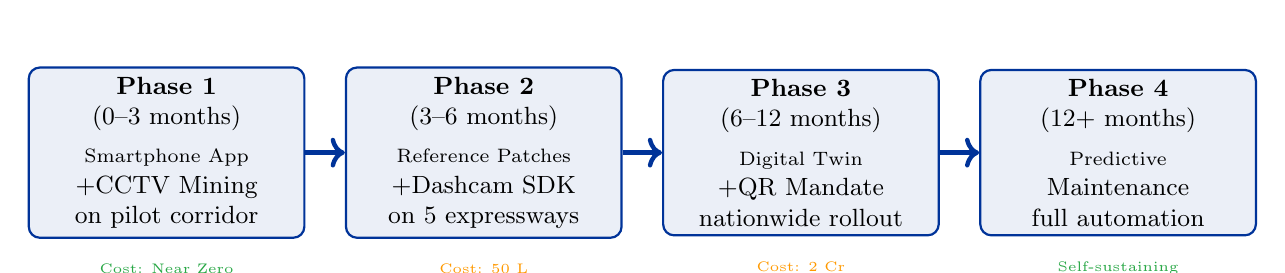
\begin{tikzpicture}[
    node distance=0.3cm,
    phase/.style={rectangle, rounded corners=4pt, draw=nhaiblue, thick, fill=nhaiblue!8, minimum width=3.5cm, minimum height=1.8cm, align=center, font=\small},
    timeline/.style={->, ultra thick, nhaiblue}
]

\node[phase] (P1) {\textbf{Phase 1}\\(0--3 months)\\[0.1cm]\scriptsize Smartphone App\\+CCTV Mining\\on pilot corridor};

\node[phase, right=0.5cm of P1] (P2) {\textbf{Phase 2}\\(3--6 months)\\[0.1cm]\scriptsize Reference Patches\\+Dashcam SDK\\on 5 expressways};

\node[phase, right=0.5cm of P2] (P3) {\textbf{Phase 3}\\(6--12 months)\\[0.1cm]\scriptsize Digital Twin\\+QR Mandate\\nationwide rollout};

\node[phase, right=0.5cm of P3] (P4) {\textbf{Phase 4}\\(12+ months)\\[0.1cm]\scriptsize Predictive\\Maintenance\\full automation};

\draw[timeline] (P1) -- (P2);
\draw[timeline] (P2) -- (P3);
\draw[timeline] (P3) -- (P4);

\node[below=0.2cm of P1, font=\tiny, text=successgreen] {Cost: Near Zero};
\node[below=0.2cm of P2, font=\tiny, text=warningorange] {Cost: 50 L};
\node[below=0.2cm of P3, font=\tiny, text=warningorange] {Cost: 2 Cr};
\node[below=0.2cm of P4, font=\tiny, text=successgreen] {Self-sustaining};
\end{tikzpicture}
\caption{Phased deployment roadmap. Phase~1 requires zero capital expenditure, enabling immediate proof-of-concept.}
\label{fig:roadmap}
\end{figure}


%==============================================================================
\section{Evaluation Against Hackathon Criteria}
\label{sec:evaluation}
%==============================================================================

\begin{table}[H]
\centering
\caption{Self-Assessment Against NHAI Hackathon Evaluation Criteria}
\label{tab:evaluation}
\begin{tabular}{@{}p{3.5cm}cp{8.5cm}@{}}
\toprule
\textbf{Criterion} & \textbf{Weight} & \textbf{How RetroGuard Addresses It} \\
\midrule
\textbf{Innovation Level} & 30 & Six novel approaches, none existing in retroreflectivity domain worldwide: smartphone retroreflectometer, CCTV mining of headlight reflections, degradation-encoding QR codes, crowdsourced dashcam network, reference patch universal calibration, predictive digital twin \\
\midrule
\textbf{Feasibility} & 30 & Layers 1--2 deployable immediately with zero hardware cost. Prototype demonstrated with working smartphone app, CCTV analysis pipeline, and web dashboard. Uses existing NHAI infrastructure (CCTV, ATMS) \\
\midrule
\textbf{Scalability \& Sustainability} & 20 & Covers 1,40,000+ km from Day~1 through existing CCTVs and crowdsourced dashcams. Self-improving: more data $\to$ better predictions. No recurring hardware costs for Layers~1--2 \\
\midrule
\textbf{Presentation \& Documentation} & 20 & Comprehensive technical paper with mathematical foundations, system architecture diagrams, flowcharts, cost-benefit analysis, and deployment roadmap. Live demo of working prototype \\
\bottomrule
\end{tabular}
\end{table}


%==============================================================================
\section{Conclusion}
\label{sec:conclusion}
%==============================================================================

\subsection{Summary}

We have presented \textbf{RetroGuard}, a comprehensive six-layer system for automated retroreflectivity assessment on Indian national highways. The system uniquely addresses all three NHAI solution categories:

\begin{enumerate}[noitemsep]
    \item \textbf{Vehicle/Drone-Mounted Measurement:} Through the crowdsourced dashcam network (Layer~4) and drone integration capability
    \item \textbf{AI/ML-Based Determination:} Through YOLOv8 detection, regression CNN estimation, LSTM degradation prediction, and CCTV intelligence mining (Layers~2, 5)
    \item \textbf{Combination:} Through the unified Digital Twin platform integrating all six layers
\end{enumerate}

\subsection{Key Differentiators}

\begin{enumerate}[noitemsep]
    \item \textbf{Zero-to-Full Coverage:} Starts with no capital investment (smartphone app + CCTV mining) and scales to continuous network-wide monitoring
    \item \textbf{Shift from Reactive to Predictive:} The Digital Twin doesn't just measure current state --- it predicts future failures, enabling proactive maintenance
    \item \textbf{Self-Improving System:} More vehicles, more time, more weather conditions all improve the prediction models automatically
    \item \textbf{Universal Calibration:} Reference patches solve the fundamental camera calibration problem for pennies, enabling any camera to become a measurement instrument
    \item \textbf{Manufacturing Integration:} QR codes make signs self-reporting, creating an asset management revolution at negligible cost
\end{enumerate}

\subsection{Potential Impact}

If deployed across NHAI's national highway network:

\begin{itemize}[noitemsep]
    \item \textbf{Coverage:} From $<$1\% to 100\% of highway safety assets monitored continuously
    \item \textbf{Response Time:} From annual/biannual inspections to real-time alerting
    \item \textbf{Cost:} From crores (mobile retroreflectometers) to lakhs (software + reference patches)
    \item \textbf{Safety:} Zero inspector exposure to highway traffic during measurement
    \item \textbf{Compliance:} Automated, continuous IRC~67/35 compliance documentation
\end{itemize}

RetroGuard transforms retroreflectivity management from a periodic, expensive, dangerous manual activity into a continuous, automated, predictive system --- ultimately contributing to the vision of safer national highways and reduced road fatalities in India.

%==============================================================================
% References
%==============================================================================

\newpage
\section*{References}
\addcontentsline{toc}{section}{References}

\begin{enumerate}[label={[\arabic*]}, noitemsep, leftmargin=*]
    \item Indian Roads Congress, \textit{IRC:67-2012 --- Code of Practice for Road Signs}, New Delhi, 2012.
    \item Indian Roads Congress, \textit{IRC:35-2015 --- Code of Practice for Road Markings}, New Delhi, 2015.
    \item Ministry of Road Transport and Highways, \textit{Road Accidents in India --- 2023}, Government of India, 2024.
    \item ASTM International, \textit{ASTM E1709-09: Standard Test Method for Measurement of Retroreflective Signs Using a Portable Retroreflectometer at a 0.2 Degree Observation Angle}, 2009.
    \item ASTM International, \textit{ASTM E1710-18: Standard Test Method for Measurement of Retroreflective Pavement Marking Materials with CEN-Prescribed Geometry Using a Portable Retroreflectometer}, 2018.
    \item Jocher, G., Chaurasia, A., Qiu, J., \textit{Ultralytics YOLO (Version 8.0)}, 2023. Available: https://github.com/ultralytics/ultralytics
    \item Zhao, Y., Lv, W., et al., ``DETRs Beat YOLOs on Real-time Object Detection,'' \textit{Proceedings of the IEEE/CVF Conference on Computer Vision and Pattern Recognition (CVPR)}, 2024.
    \item Carlson, P.J., Park, E.S., Andersen, C.K., ``The Benefits of Pavement Markings: A Renewed Perspective Based on Recent and Ongoing Research,'' \textit{Transportation Research Record}, vol.~2107, pp.~59--68, 2009.
    \item Federal Highway Administration, \textit{Retroreflectivity of Pavement Markings: NCHRP Synthesis 306}, Transportation Research Board, 2003.
    \item Zwahlen, H.T., Schnell, T., ``Visibility of Road Markings as a Function of Age, Retroreflectivity Under Low-Beam and High-Beam Illumination at Night,'' \textit{Transportation Research Record}, vol.~1692, pp.~152--163, 1999.
    \item Burns, D.M., et al., ``Mobile Retroreflectivity Measurement for Pavement Markings,'' \textit{Transportation Research Record}, vol.~2055, pp.~60--70, 2008.
    \item Hochreiter, S., Schmidhuber, J., ``Long Short-Term Memory,'' \textit{Neural Computation}, vol.~9, no.~8, pp.~1735--1780, 1997.
    \item He, K., Zhang, X., Ren, S., Sun, J., ``Deep Residual Learning for Image Recognition,'' \textit{Proceedings of the IEEE Conference on Computer Vision and Pattern Recognition}, pp.~770--778, 2016.
\end{enumerate}

%==============================================================================
% Appendices
%==============================================================================

\newpage
\appendix

\section{API Specification for RetroGuard Cloud Platform}

\begin{lstlisting}
# RetroGuard API - Core Endpoints

# Submit a retroreflectivity measurement
POST /api/v1/measurements
{
    "asset_type": "sign|marking|rpm|delineator",
    "gps_lat": 19.0760,
    "gps_lon": 72.8777,
    "highway_id": "NH-48",
    "chainage_km": 234.5,
    "rl_estimated": 145.3,
    "confidence": 0.87,
    "source_layer": "smartphone|cctv|dashcam",
    "image_hash": "sha256:...",
    "conditions": {
        "time": "night",
        "weather": "dry",
        "streetlight": false
    },
    "device_info": {
        "model": "Samsung Galaxy S24",
        "calibration_date": "2026-04-01"
    }
}

# Query asset health
GET /api/v1/assets/{asset_id}/health
Response: {
    "current_rl": 145.3,
    "irc_minimum": 150,
    "status": "warning",
    "predicted_failure_date": "2026-06-15",
    "confidence": 0.82,
    "recommendation": "Schedule replacement within 60 days"
}

# Generate compliance report
GET /api/v1/reports/compliance?highway=NH-48&from_km=200&to_km=300
Response: PDF report per IRC 67/35 standards
\end{lstlisting}

\section{Smartphone Calibration Algorithm}

\begin{algorithm}[H]
\caption{Smartphone Retroreflectivity Calibration and Measurement}
\label{alg:calibration}
\begin{algorithmic}[1]
\Require Reference patch with known $R_{L,ref}$, smartphone with RAW capture
\Ensure Calibrated retroreflectivity measurement $\hat{R}_L$

\Statex \textbf{--- Calibration Phase (once per session) ---}
\State Position phone at distance $d_{cal}$ from reference patch
\State Capture RAW image with flash ON: $I_{flash}$
\State Capture RAW image with flash OFF: $I_{ambient}$
\State $P_{ref} \gets \text{mean}(I_{flash} - I_{ambient})$ over patch region
\State $K_{cal} \gets R_{L,ref} / P_{ref}$ \Comment{Calibration constant}

\Statex
\Statex \textbf{--- Measurement Phase (per target) ---}
\State Aim phone at target sign/marking
\State Capture RAW image pair (flash ON/OFF)
\State Run YOLOv8 detection to identify target region
\State $P_{target} \gets \text{mean}(I_{flash} - I_{ambient})$ over target region
\State Estimate distance $d_{target}$ via known sign size or LiDAR
\State Compute geometric correction: $G = (d_{target}/d_{cal})^2 \cdot (\cos\beta_{cal}/\cos\beta_{target})$
\State $\hat{R}_L \gets K_{cal} \cdot P_{target} \cdot G$

\Statex
\Statex \textbf{--- Quality Check ---}
\If{$\text{SNR}(P_{target}) < 20\text{ dB}$}
    \State \textbf{flag} ``Low confidence --- retake measurement''
\EndIf
\State \Return $\hat{R}_L$, confidence, GPS, timestamp
\end{algorithmic}
\end{algorithm}

\end{document}
